\documentclass[11pt,a4paper]{article}
\usepackage[T1]{fontenc}
\usepackage[utf8]{inputenc}
\usepackage{lmodern}
\usepackage[margin=23mm,headheight=14pt]{geometry}
\usepackage{microtype,amsmath,amssymb,booktabs,tabularx,array,graphicx}
\usepackage[font=small,labelfont=bf]{caption}
\usepackage[numbers,sort&compress]{natbib}
\usepackage{xcolor,enumitem,fancyhdr,placeins,url}
\usepackage[colorlinks=true,linkcolor=blue!45!black,citecolor=blue!45!black,urlcolor=blue!45!black,breaklinks=true]{hyperref}
\hypersetup{pdftitle={Thresholds and Learning in Adaptive Intrusion Detection: A Two-Capture Case Study},pdfauthor={Oleksandr Kuznetsov; Emanuele Pio De Bernardis},pdfsubject={Revised manuscript with post-review experiments, 1 November 2026},pdfkeywords={intrusion detection, concept drift, delayed labels, threshold adaptation, additive splines, TON IoT, UNSW-NB15}}
\setlength{\parindent}{1.2em}
\setlength{\parskip}{3pt}
\linespread{1.04}
\setlist{nosep,leftmargin=*}
\setlength{\emergencystretch}{2em}
\pagestyle{fancy}\fancyhf{}
\fancyhead[L]{\small Thresholds and learning in intrusion detection}
\fancyhead[R]{\small Revised manuscript}
\fancyfoot[C]{\thepage}
\newcommand{\F}{\textsc{Frozen}}
\newcommand{\FIT}{\textsc{Fit192}}
\newcommand{\CAL}{\textsc{Cal64}}
\newcommand{\code}[1]{\texttt{\detokenize{#1}}}
\newcommand{\pp}{\,\mathrm{pp}}
\newcommand{\meanauc}{\overline{\mathrm{AUC}}_{\mathrm{block}}}
\makeatletter
\setlength{\@fptop}{0pt}
\setlength{\@fpsep}{14pt}
\setlength{\@fpbot}{0pt plus 1fil}
\newcommand{\tablerows}[1]{\@@input #1 }
\makeatother

\hypersetup{pdftitle={Thresholds and Learning in Adaptive Intrusion Detection: A Two-Capture Case Study},pdfsubject={Second-review revision, 1 November 2026}}
\title{\vspace{-12mm}\textbf{Thresholds and Learning in Adaptive Intrusion Detection: A Two-Capture Case Study}}
\author{Oleksandr Kuznetsov$^{1,2,*}$ \quad Emanuele Pio De Bernardis$^{1}$\\[5pt]
\small $^{1}$Department of Theoretical and Applied Sciences, eCampus University,\\[-2pt]
\small Via Isimbardi 10, 22060 Novedrate (CO), Italy\\[3pt]
\small $^{2}$Department of Intelligent Software Systems and Technologies,\\[-2pt]
\small School of Computer Science and Artificial Intelligence,\\[-2pt]
\small V. N. Karazin Kharkiv National University, 4 Svobody Sq., 61022 Kharkiv, Ukraine\\[5pt]
\small $^{*}$Correspondence: \href{mailto:oleksandr.kuznetsov@uniecampus.it}{oleksandr.kuznetsov@uniecampus.it}\\[3pt]
\small ORCID: \href{https://orcid.org/0000-0003-2331-6326}{0000-0003-2331-6326} (O.K.); \href{https://orcid.org/0009-0004-7915-5204}{0009-0004-7915-5204} (E.P.D.B.)}

\date{1 November 2026 --- second-review revision}
\begin{document}
\maketitle\thispagestyle{plain}
\begin{abstract}
An adaptive intrusion detector can change its score function, its decision threshold, or both. We examine their separate contributions under sparse, delayed supervision in two recorded network captures. Paired chronological replays hold label requests and feedback timing fixed, while varying learning, calibration memory, and threshold objectives. In TON\_IoT, a spline head reduces the false-positive rate by 28.36 percentage points relative to a frozen detector when both thresholds maximize recent balanced accuracy. This comparison is sensitive to the operating policy: doubling the false-positive weight raises the frozen detector's balanced accuracy from 72.12\% to 86.78\%, exceeding the head's 84.84\% at the original weight; the head reaches 87.55\% at the doubled weight. On UNSW-NB15, the historical frozen spline achieves 96.29\% balanced accuracy, above both recent threshold adaptation and head refitting. Additional diagnostics examine matched-error operating points, calibration FPR targets, precision--recall, model initialization, and controller sensitivity. Poor transfer of logistic regression and degeneration of chronological forest initializations qualify comparisons against their frozen controls. Shuffled forest initialization preserves a TON learning benefit at a common error rate, while its frozen historical policy is stronger on UNSW. Five seeds quantify algorithmic variation conditional on each recorded stream. The contribution is a reproducible case study showing how threshold policy, score quality, and effective label use jointly determine the apparent benefit of adaptation.
\end{abstract}
\noindent\textbf{Keywords:} intrusion detection; delayed labels; threshold selection; error trade-offs; temporal evaluation; reproducibility.

\section{Introduction}
An intrusion detector assigns a score to each observation and compares it with a decision threshold. Updating the score and moving the threshold are different interventions. Either can change the number of missed attacks and false alarms. A comparison of adaptive and static detectors therefore needs to establish which intervention supplies the reported improvement.

This question becomes more difficult when labels are scarce and delayed. The observations available for refitting may differ from those available for threshold selection. A small calibration memory can favor a different operating point from a larger memory, even when both optimize the same objective. Furthermore, a frozen model can be a weak reference because its initial fit transfers poorly to the evaluation period. These effects can make a large adaptive-versus-frozen contrast misleading as evidence of general learning superiority.

We study these issues using chronological TON\_IoT and UNSW-NB15 replays. The principal question is: \emph{what improvement remains after specifying a strong threshold-only controller, a relevant operating point, and a clear label-use contract?} The model families are an additive spline detector, logistic regression (LR), and an adaptive random forest (ARF). The spline intervention refits only eight feature gains and an intercept, providing a compact, explicit change to the score function.

The evidence has a defined scope. The historical TON campaign supplies an archived four-trace experiment. Subsequent controls and the present diagnostics were motivated by its observed outcomes. Both extensions are exploratory on TON. UNSW is a separate controlled capture, but had appeared elsewhere in the project. Neither capture is an untouched prospective field test. All reported seed variation is conditional on one stream per dataset.

The main contribution is the joint evaluation of score adaptation, causal threshold selection, label use, and representation recurrence. The results below emphasize operating policies and baseline quality. The Supplement retains the full historical campaign, implementation details, attack-family results, resource accounting, and sensitivity tables.

\section{Related work}
Concept-drift research distinguishes changes in a data-generating process from the mechanisms used to detect or respond to them \citep{gama2014}. Prequential evaluation requires prediction before an observation is used for learning \citep{gama2013}; delayed-label evaluation makes the feedback schedule explicit \citep{grzenda2020}. Adaptive random forests combine online ensembles with drift-triggered replacement \citep{gomes2017}. Active learning addresses the separate question of which labels to request \citep{zliobaite2014}. We use uniform requests so that acquisition remains fixed across controllers.

In security, INSOMNIA combines adaptation with active learning and label estimation \citep{andresini2021}; continuous Android malware learning similarly couples representation updates and selective labeling \citep{chen2023}. Transcend and CADE study drift detection and explanation \citep{jordaney2017,yang2021}. Our focus is the downstream attribution of decision changes once feedback is available. Temporal and spatial biases, deployment assumptions, and dataset construction remain central to this interpretation \citep{pendlebury2019,arp2022,sommer2010,engelen2021}.

Threshold selection differs from probability calibration \citep{guo2017}. Here CAL denotes examples used to select a binary threshold, without asserting that scores are posterior probabilities. Prior-shift correction provides an intercept-based reference \citep{saerens2002,lipton2018}, while changing class-conditional traffic can require more than an intercept. The spline score is a logistic generalized additive model \citep{hastie1986}; its fixed univariate representation also relates to neural additive models and KANs \citep{agarwal2021,liu2025}. The study evaluates update policies rather than proposing a new architecture.

\section{Data and causal evaluation}
\subsection{Captures, partitions, and feature availability}
TON\_IoT supplies network records from a controlled IoT/IIoT environment \citep{moustafa2021,booij2022}. We retain eight complete-flow numerical features: duration, source/destination bytes, missed bytes, and source/destination packet and IP-byte counts. Records are ordered by start time plus duration. A fits the initial transformation and model, B selects historical thresholds, C supports the original development, and D is evaluated. The full dates, preprocessing counts, and earlier structural exposure are recorded in Supplement S1.

UNSW-NB15 supplies a separately collected laboratory capture \citep{moustafa2015unsw,moustafa2016unsw}. We use its four full network CSVs, remove only three verified duplicate file-boundary rows, and retain 2,540,044 records. The eight numerical fields are \code{dur}, \code{sbytes}, \code{dbytes}, \code{sloss}, \code{dloss}, \code{Spkts}, \code{Dpkts}, and \code{tcprtt}. This is a compact feature contract with different semantics from TON. Records are sorted by $\max(\mathrm{Ltime},\mathrm{Stime}+\mathrm{float32}(\mathrm{dur}))$, then stable row identity, and split chronologically 40\%/20\%/40\% into A/B/D. Equal timestamps at boundaries are retained without an embargo. Models are fitted anew on each dataset.

\begin{table}[tb]
\centering\small
\caption{Evaluation streams. Observed prevalence is retained. Each dataset supplies one recorded stream, shared by all five algorithmic seeds.}
\label{tab:data}
\begin{tabular}{lrrrr}
\toprule
Stream & D records & Normal & Attacks & Hours \\
\midrule
TON\_IoT & 3,549,973 & 309,673 & 3,240,300 & 62.77 \\
UNSW-NB15 & 1,016,018 & 803,736 & 212,282 & 7.89 \\
\bottomrule
\end{tabular}
\end{table}

\subsection{Models, feedback, and memory}
All models use a fixed $\log(1+\max(x,0))$ transformation and standardization fitted on A. The initial LR and spline fits use the same seeded 400,000-row sample of A. LR uses the eight transformed inputs. The spline model fits eight cubic B-spline basis coefficients per feature, with subsequent adaptation restricted to
\begin{equation}
 s(x;g,b)=b+\sum_{j=1}^{8}g_j f_j(x_j),
\end{equation}
where the eight functions $f_j$ remain fixed. A head update fits eight gains and an intercept by regularized logistic regression on the current FIT memory. The original refit uses zero-centred L2 regularization; a previous-head-centred alternative is retained in the Supplement.

The stream is predicted in 10,000-row blocks. Uniform requests select 1\% of each block without replacement. Requested labels from block $k$ arrive after prediction of block $k+1$ and first affect block $k+2$. The last incomplete block is retained. All methods use the same requested row identities within a dataset, seed, delay, and budget condition. The current sampler uses \code{SeedSequence([seed, block, 20261101])}. The archived campaign's older sampler is used only in its separate numerical bridge.

A salted hash of each raw feature vector assigns it permanently to FIT or CAL with nominal probabilities 3/4 and 1/4. The default memories hold 192 FIT and 64 CAL observations, with equal per-class quotas. Repeated observations can occupy separate positions. CAL entries are eligible for 50 blocks from observation time; at least five observations of each class are required. FIT has no age filter. A head and its matched threshold change atomically only when the transaction is valid. A separate CAL256 memory accepts all requested labels and updates a frozen detector's threshold independently.

\begin{table}[tb]
\centering\small
\caption{Information contracts. All rows share acquisition and feedback timing. Model state and pending labels are additional to the listed example memories.}
\label{tab:contracts}
\begin{tabularx}{\linewidth}{lXX}
\toprule
Controller & Learning & Threshold selection \\
\midrule
Frozen / B & A only & Historical B \\
Frozen / CAL256 & A only & All requested labels; recent CAL256 \\
Head / CAL64 & Disjoint FIT192 & Recent CAL64; valid head transaction \\
ARF / CAL64 or CAL256 & Every arriving requested label & CAL labels reused in learning \\
ARF FIT-only / CAL64 & Arriving FIT-role labels only & Disjoint CAL64 \\
\bottomrule
\end{tabularx}
\end{table}

ARF uses River 0.22.0, ten trees, and defaults apart from the seed \citep{riverdocs}. The first extension processes the A sample chronologically. The present audit additionally fits the identical sample in its seeded random order. Both initial states are evaluated frozen and with feedback. The FIT-only variant starts from the chronological state and excludes every CAL-role label from learning. This aligns label disjointness with the head experiment, while retaining the forest's persistent tree memory. It does not impose the finite FIT192 retention contract. Thus ARF is an equal-acquisition-budget comparator with explicitly different model state and, for its standard variant, different label reuse.

\subsection{Threshold objectives and matched-error descriptions}
A decision is positive when $s(x)>\tau$. The historical and recent thresholds minimize
\begin{equation}
 L_\lambda(\tau)=\mathrm{FNR}(\tau)+\lambda\,\mathrm{FPR}(\tau).
 \label{eq:cost}
\end{equation}
The first extension fixes $\lambda\in\{0.25,0.5,1,2,4\}$; the current audit adds 0.75, 1.25, 1.5, and 3. Every threshold is fitted using past available labels. At $\lambda=1$, this is equivalent to maximizing balanced accuracy (BA). Exact candidate and tie rules appear in Supplement S1. For attack prevalence $\pi$ and costs $C_{\rm FN},C_{\rm FP}$, the rate weight is $C_{\rm FP}(1-\pi)/(C_{\rm FN}\pi)$. A value of one is a declared evaluation objective, rather than a universal operational cost.

Two complementary checks address operating-point comparability. First, we interpolate the observed FPR/recall polylines within their support, separately for each paired seed. This is a retrospective description of recorded policies. It neither selects a deployable threshold nor estimates an oracle ROC curve. Interpolating a curve of seed means is also reported and kept distinct from averaging the paired-seed comparisons.

Second, causal FPR-target controllers use only past normal calibration scores. For target $\alpha\in\{0.05,0.10,0.20\}$, they select the smallest observed negative-score threshold with empirical FPR at most $\alpha$, respecting complete ties. B supplies the initial threshold. The frozen score uses CAL256, and the head uses its disjoint CAL memory. Requested targets are identical; achieved future FPR can differ under distribution change. We report both achieved FPR and recall rather than assuming that a calibration target is a future guarantee.

\subsection{Metrics, overlap, and evidence status}
We sum confusion counts over D before calculating recall, FPR, BA, and precision. AUROC and noninterpolated average precision (AP) are also calculated within prediction blocks containing both classes. We report macro, normal-count-weighted, and attack-count-weighted summaries and their coverage. Pooled AUROC/AP are used only for a fixed score. Pooling adaptive scores would compare values from different fitted states. AP is the recall-increment-weighted mean of precision, as implemented by scikit-learn, rather than a trapezoidal interpolation \citep{pedregosa2011,sklearnap}.

Seen/unseen strata refer to exact equality of eight stored float32 features against earlier A/B/C vectors on TON and A/B vectors on UNSW. They describe representation recurrence, not event identity, attack-family novelty, or memorization. Both strata are evaluated on the same adaptive trajectory.

Seeds 42--46 vary the initial sample and label requests. All seed means and sample SDs are \emph{conditional on the same recorded stream}; five seeds are not five independent captures. The historical acceptance rule required joint non-increase of FN and FP, with at least one strict improvement, in four of five spline seeds against Frozen/CAL64. It was a versioned empirical rule, not an externally registered trial or significance test. Analogous counts for other models and controls are exploratory. Original results, first-extension results, and new diagnostics are retained separately.

\section{Results}
\subsection{The apparent head benefit depends on threshold policy}
Table~\ref{tab:costs} contains the central comparison. On TON at $\lambda=1$, the spline head lowers FPR by 28.36 percentage points and recall by 2.92 points relative to Frozen/CAL256. Each seed has fewer FP and more FN. This is a difference between two complete update policies at one declared calibration objective.

Changing only the frozen detector's cost weight to $\lambda=2$ raises its BA from 72.12\% to 86.78\%, above the head's 84.84\% at $\lambda=1$. At $\lambda=2$, the head reaches 87.55\% BA. The large 28-point FPR contrast therefore cannot be interpreted as a comparable advantage across operating points. The observed operating curves in Figure~\ref{fig:costs} show where the gap changes.

\begin{table}[tb]
\centering\small\setlength{\tabcolsep}{4pt}
\caption{Spline operating policies. Rates are percentages, mean $\pm$ sample SD across five randomizations conditional on each stream. Each threshold uses only past labels.}
\label{tab:costs}
\begin{tabular}{llrrr}\toprule
Stream & Policy & Recall & FPR & BA \\\midrule
\tablerows{tables/review2_cost_rows.tex}
\bottomrule\end{tabular}
\end{table}

\begin{figure}[tb]
\centering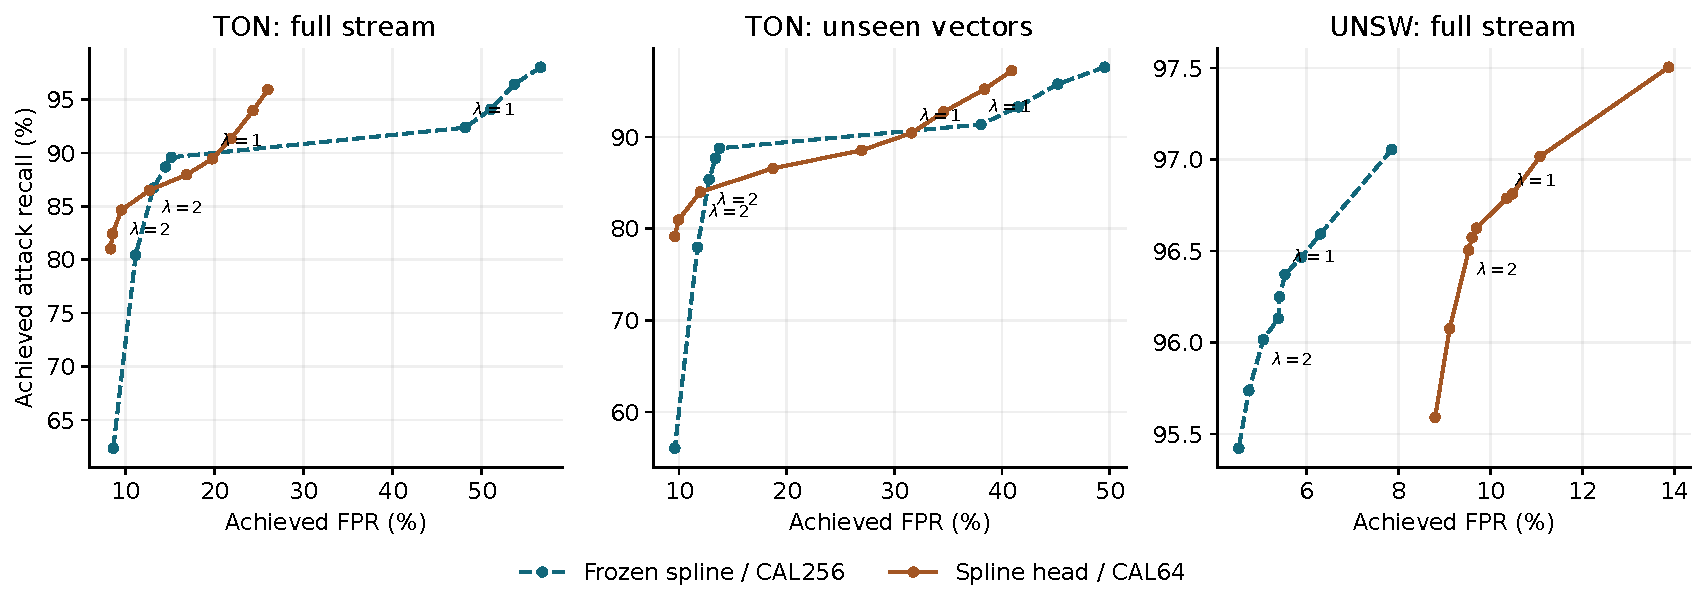
\includegraphics[width=\linewidth]{figures/review2_operating_points.pdf}
\caption{Causal threshold policies for the fixed cost grid. Points are means over five paired randomizations on each single stream. Lines connect implemented policies and do not constitute an oracle frontier. Axis ranges differ. The annotated weights illustrate why a single $\lambda=1$ contrast cannot establish curve-wide superiority.}
\label{fig:costs}
\end{figure}

The original five-point grid also makes interpolation resolution important. In TON seed 42, the frozen thresholds at $\lambda=0.25$ and 0.5 coincide in 238 of 355 blocks; those at 2 and 4 coincide in 201. Finite calibration data produce shared thresholds and coarse operating points. Supplement S4 provides each seed and distinguishes interpolation of the mean curve from paired-seed interpolation. The latter retains variation in the location of the operating points; the two summaries need not agree.

With the denser nine-weight grid, the paired head-minus-frozen recall difference at 13\% FPR is $1.49 \pm 3.66$ percentage points (5 supported pairs). This remains a retrospective interpolation within each seed, rather than a threshold selected for a new stream.


On UNSW, the historical Frozen/B spline is strongest by mean BA among the default spline policies: 96.29\%. Recent CAL64 selection lowers BA to 93.75\%, CAL256 to 95.42\%, and head/CAL64 to 93.22\%. Thus neither tested recent threshold adaptation nor head refitting improves BA over the historical policy on this capture. A higher recall under another policy remains possible at a larger false-alarm cost. This qualifies any claim that adaptation generally fails or succeeds independently of the chosen utility.

\subsection{Calibration targets and precision--recall}
Table~\ref{tab:fprtargets} evaluates common calibration FPR targets. These controllers supply a causal check independent of the $\lambda=1$ objective. Their realized FPRs must be examined before comparing recall: the same calibration target can produce different future false-alarm burdens. In particular, a small CAL64 sample and a changed score can miss the requested target substantially.

\begin{table}[tb]
\centering\small\setlength{\tabcolsep}{4pt}
\caption{Requested calibration FPR versus achieved future rates for the spline score. Target and rates are percentages. Mean $\pm$ sample SD describes five randomizations of the same stream. Thresholds use only previously available normal labels.}
\label{tab:fprtargets}
\begin{tabular}{lr l rrr}\toprule
Stream & Target & Controller & Recall & FPR & BA \\\midrule
\tablerows{tables/review2_fpr_rows.tex}
\bottomrule\end{tabular}
\end{table}

The $\lambda=1$ contrast alone cannot diagnose sampling noise as the cause. On TON, weighting valid calibration/next-block pairs by the next block's normal count gives calibration FPR 42.67\% and subsequent FPR 48.30\% at $\lambda=1$, versus 8.26\% and 13.20\% at $\lambda=2$. Thus the selected calibration policy already accepts many false alarms; the subsequent rates also reflect transfer. The diagnostic supplement compares calibration and subsequent-block errors and records the number of distinct normal scores. These measurements separate a policy that accepts many false alarms in its calibration objective from one that violates an intended FPR target after transfer. They do not identify a unique causal source of the observed shift.

Figure~\ref{fig:pr} reports precision--recall at the actual causal operating points. TON's attack-dominated prevalence can yield high precision despite a large FPR. To make that dependence visible, the third panel uses the same class-conditional rates at hypothetical 1\% prevalence:
\begin{equation}
 \mathrm{precision}(\pi)=\frac{\pi\,\mathrm{recall}}{\pi\,\mathrm{recall}+(1-\pi)\,\mathrm{FPR}}.
\end{equation}
For example, the TON head at $\lambda=1$ yields 4.37\% precision at 1\% prevalence and 0.45\% at 0.1\%. These are conditional calculations, not predictions for a new network.

\begin{figure}[tb]
\centering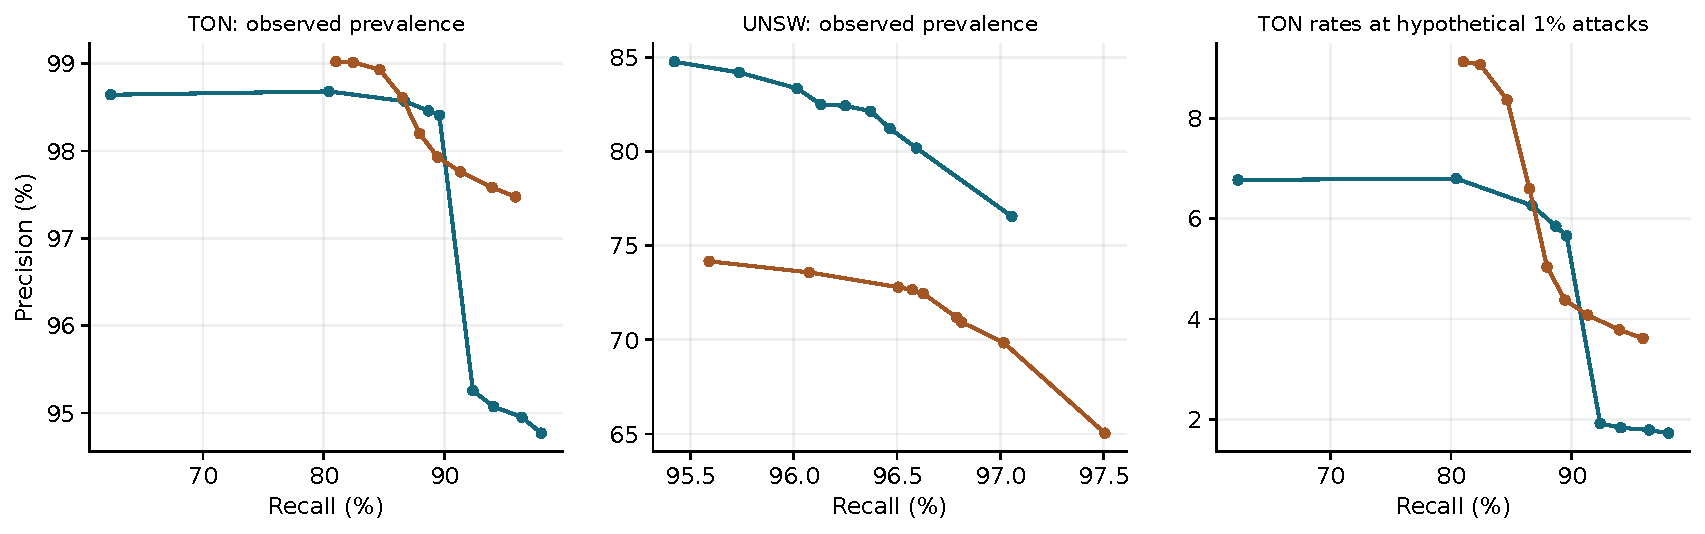
\includegraphics[width=\linewidth]{figures/review2_precision_recall.pdf}
\caption{Precision--recall operating points selected by the fixed cost grid. The first two panels use observed class counts. The last panel assumes that TON's class-conditional rates transfer to 1\% attack prevalence. Points are seed means conditional on each capture; they are not pooled adaptive-score PR curves.}
\label{fig:pr}
\end{figure}

\subsection{Baseline quality changes the interpretation of learning}
The frozen LR on TON has pooled D AUROC 0.318 and Frozen/B BA 25.50\%. We therefore audited attack-label orientation, the coefficient score, \code{decision_function}, attack probabilities, optimization convergence, and the cached score. The fixed-score A/B/D diagnostics are in Table~\ref{tab:audit}. An inversion on B or D is an observed transfer failure; it is not repaired by reversing scores using D labels. Consequently, the poor frozen LR is retained as a failure case rather than presented as a strong performance comparator.

\begin{table}[tb]
\centering\small
\caption{Initial-model audit: pooled AUROC, mean $\pm$ seed SD conditional on each capture. A describes the training population and is not an out-of-sample estimate. The chronological and shuffled forests use the same sampled A rows.}
\label{tab:audit}
\begin{tabular}{llrrr}\toprule
Stream & Initial model & A & B & D \\\midrule
\tablerows{tables/review2_audit_rows.tex}
\bottomrule\end{tabular}
\end{table}

Against its own Frozen/CAL256 control, the TON LR head reduces FP in all five seeds and FN in four. The exception is seed 45, with 62,138 additional FN. This is an exploratory 4/5 joint-improvement count for a different learner and comparator; it does not overturn the failed historical spline criterion. Its interpretation also depends on the frozen LR's poor ranking. Similar head BA values for LR and splines conceal different starting points and error changes.

The initial chronological forest is also weak. On UNSW, seed 43 has a constant score, AUROC 0.5, and recall and FPR of 100\% at the historical threshold. Three other seeds have inverted pooled ranking. TON's frozen forest has pooled AUROC 0.40--0.46. Large adaptive-versus-frozen differences against these states cannot alone establish the superiority of a richer learner. Table~\ref{tab:arf} therefore includes the shuffled-A initialization and the disjoint-label feedback control, while retaining the original chronological results.

\begin{table}[tb]
\centering\fontsize{8.7}{10.5}\selectfont\setlength{\tabcolsep}{3pt}
\caption{Forest diagnostics, percentages as mean $\pm$ SD across five randomizations conditional on each capture. All policies share acquired labels; FIT-only uses a subset for learning and disjoint CAL64. Tree state is persistent and is not constrained to the head's example-memory contract.}
\label{tab:arf}
\begin{tabular}{lllrrr}\toprule
Stream & Initial/feedback condition & Policy & Recall & FPR & BA \\\midrule
\tablerows{tables/review2_arf_rows.tex}
\bottomrule\end{tabular}
\end{table}

For the original chronological initialization, adaptive ARF/CAL256 reaches 90.39\% BA on TON, compared with 86.78\% for spline Frozen/CAL256 at $\lambda=2$ and 87.55\% for the spline head at $\lambda=2$. On UNSW it reaches 95.86\%, close to spline Frozen/CAL256 at $\lambda=1$ (95.42\%) and below spline Frozen/B (96.29\%). These are descriptive comparisons among the evaluated policies at equal acquisition budgets. Their different retained state and effective label use remain part of the result.

On TON, shuffled-A ARF/CAL256 reaches 89.94\% BA; its corresponding frozen/CAL256 state reaches 73.67\%, and its historical frozen/B policy reaches 57.78\%. The chronological FIT-only/CAL64 forest reaches 87.43\%, using CAL-role labels exclusively for threshold selection.

On UNSW, shuffled-A ARF/CAL256 reaches 96.74\% BA; its corresponding frozen/CAL256 state reaches 96.94\%, and its historical frozen/B policy reaches 97.84\%. The chronological FIT-only/CAL64 forest reaches 94.32\%, using CAL-role labels exclusively for threshold selection.

At 20\% FPR, within-seed interpolation of the shuffled forests' nine-weight policies gives adaptive-minus-frozen recall $18.24 \pm 13.88$ percentage points across all five supported pairs. This comparison uses adaptive CAL64 versus frozen CAL256, and the forest retains persistent state and calibration-label reuse. It supports a TON learning contribution under that contract beyond the spline-specific single-point contrast. The selected matched-FPR targets have no common support for all five UNSW pairs; no extrapolated forest comparison is used there.

These initialization and label-use contrasts delimit the forest result. The shuffled initial state is a batch-initialization control on historical A, not a reshuffling of the evaluation stream. The FIT-only control removes calibration-label reuse during D while preserving the forest's accumulated tree state; it supplies a label-use check rather than an equal-memory comparison.


\begin{figure}[tb]\centering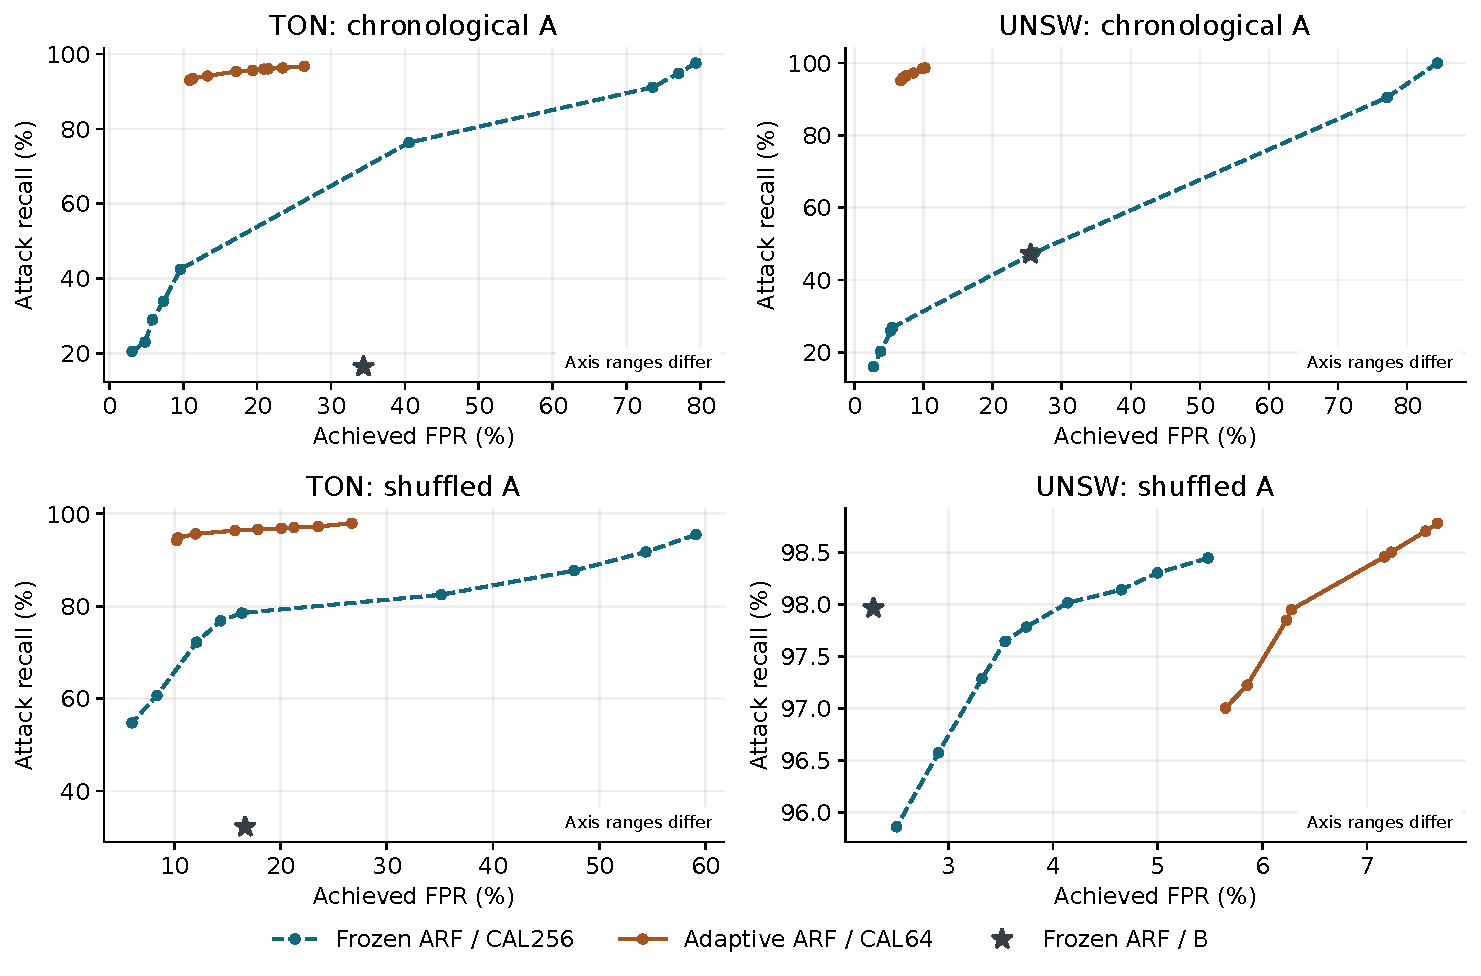
\includegraphics[width=\linewidth]{figures/review2_forest_operating_points.pdf}
\caption{Forest operating policies under chronological and shuffled historical initialization. Connected points use the nine fixed cost weights, with thresholds selected from past labels. Stars mark the fixed historical B threshold. Means describe five randomizations on each stream; axis ranges differ. The frozen control uses CAL256 and the adaptive forest CAL64; the standard forest reuses CAL labels for learning and retains persistent tree state.}
\label{fig:forest}
\end{figure}
Figure~\ref{fig:forest} places the forest comparisons in their operating regions. The historical-threshold point can outperform recent calibration on stable ranking, while an adaptive policy can help after poor transfer. A comparison at one weight, including an ARF comparison, remains a statement about the specified complete policies. The Supplement's CSV includes paired matched-error descriptions for these forests as well.


\subsection{Ranking heterogeneity and controller sensitivity}
The frozen spline's TON macro block AUROC is 0.850, while weighting valid blocks by their normal counts gives 0.557. Blocks with few normal observations have disproportionate influence on the macro summary relative to their contribution to false-alarm workload. The normal-weighted statistic exposes weak average within-block separation under that weighting. It does not imply that every normal-heavy block is near chance, nor does AUROC alone determine FPR at a selected threshold. Both summaries, pooled fixed-score AUROC, blockwise AP, and coverage are retained in Supplement S4.

Controller robustness is assessed one factor at a time on both captures: FIT/CAL capacities 96/32 and 384/128; calibration ages 10 and 100 blocks; a minimum of ten CAL examples per class; and two additional fixed role salts. All five seeds are retained for every setting. These checks assess the declared controller rather than selecting a new best configuration. They complement the earlier TON delay and budget tests: at a 0.1\% query budget the default spline head reaches 57.49\% BA, compared with 79.48\% for Frozen/CAL256. Detailed rates, update counts, and conditional variation are reported in the Supplement.

On TON, head BA across the eight declared settings ranges from 81.49\% to 88.97\%. The default and the two alternative role salts yield 84.84\%, 83.95\%, and 88.97\%, respectively. On UNSW, head BA across the eight declared settings ranges from 89.63\% to 93.89\%. The default and the two alternative role salts yield 93.22\%, 92.44\%, and 89.63\%, respectively.

The salt dependence is substantial and differs between captures. A favorable individual partition should therefore not be reported as a stable model advantage. Across these eight head settings, UNSW BA remains below the historical frozen spline.

\subsection{Historical Stage 1 and its numerical sensitivity}
The archived TON campaign established the original motivation. With a frozen score, recent CAL64 raises recall from 21.11\% to 89.09\%, while FPR rises from 12.64\% to 46.74\%. Adding head refitting gives recall 89.38\% and FPR 20.47\%. Of the FP reduction, 96.7\% occurs on vectors previously observed in A/B/C, where recall decreases. The full-stream FN mean combines opposing seen/unseen changes. Only seeds 43, 45, and 46 improve both error counts, so the specified 4/5 criterion fails.

The same-query Linux numerical bridge changes that count from 3/5 to 2/5. Its paired FN differences are $+33{,}457$, $-115{,}004$, $+123{,}984$, $-45{,}794$, and $+47{,}576$ for seeds 42--46, respectively. The seed-46 change is largely associated with its frozen calibration trace. This sensitivity is evidence against treating a seed-count cutoff as an inferential conclusion. The original measurements remain historical evidence; the bridge is a separately fitted reconstruction, not bitwise replication. Full counts and provenance appear in Supplement S2--S3.

\section{Discussion and limits}
The defensible conclusion concerns the complete decision policy. Equal $\lambda$ comparisons are meaningful tests of two specified calibration procedures, but they cannot establish uniform superiority of their score functions. Matched-error descriptions and causal FPR-target controllers answer complementary questions. A strong evaluation should report the operating region, actual achieved rates, effective calibration evidence, and the quality of the frozen reference.

The overlap result is similarly conditional. The first extension's $\lambda=1$ spline comparison locates 90.5\% of FP savings on previously seen vectors. This percentage describes where that policy saves false alarms. It is not the fraction of benefit caused by memorization, and it changes when the control or operating objective changes. Exact feature equality can merge distinct flows and miss near-duplicates. A tolerance-based or host/session analysis would require a separately justified identity definition; it is outside the present eight-feature recurrence claim.

The two captures support controlled case-study conclusions. They do not estimate effectiveness across operational networks. Seed SDs, block summaries, and historical moving-block resampling all condition on the recorded streams. The original D structural checks and earlier project exposure are disclosed; new protocols and runner hashes are fixed before their respective diagnostic executions. Holding D labels out of controller decisions prevents look-ahead within replay, while the broader exploratory research history remains.

Feedback is also an assumption. At the 1\% budget, TON requires approximately 566 labels per recorded hour and UNSW approximately 1,288. Block-delay medians are about 3.50 and 6.45 minutes, respectively. These volumes and delays describe an annotation service, not a demonstrated analyst workflow. Labels are treated as correct. Active acquisition, noisy or asynchronous analyst feedback, and operational capacity estimation require new experiments. A deployment-specific $\lambda$ should be set from past evidence and declared costs or capacity, with an evaluation period kept separate.

Reproducibility has two levels. Original Windows reports are preserved and reanalyzed exactly, while the available Linux reconstruction does not reproduce every initial fit or prediction. The new extensions retain initial models, source hashes, input-array digests, full per-block reports, and pinned dependencies so that their recorded analyses and causal replays can be checked. A Git revision identifies the implementation; long-term archival deposition is a separate obligation.

\section{Conclusions}
Threshold policy materially changes the apparent value of score adaptation in these two captures. On TON, the large spline-head advantage at a single balanced-accuracy calibration point narrows or changes across operating regions. On UNSW, the historical frozen spline has higher mean BA than the tested default threshold or head updates. Weak frozen LR and forest initializations further show why an adaptive-versus-frozen difference requires a baseline-quality audit. After shuffled initialization, the forest retains a TON advantage at a common FPR under its more permissive state and label-use contract. On UNSW, its frozen historical policy has higher BA than its tested recent-threshold and learning policies. The two captures therefore support model- and policy-specific conclusions.

The useful output is a reproducible evaluation procedure: match acquisition and feedback, disclose effective label use and retained state, examine more than one operating point, audit initial scores, and separate algorithmic randomization from independent-stream evidence. These checks support specific claims about error compromises and identify which broader claims would need new captures.

\section*{Data and code availability}
TON\_IoT and UNSW-NB15 are used under their providers' academic-use conditions \citep{toniotweb,unswweb}. Raw network data are not redistributed. Source hashes, parser versions, and attribution details are supplied with the code and in the Supplement. The historical executed commit is \code{ea21691}, with retained evidence at \code{81d99d9}. First-extension code and results are at \href{https://github.com/KuznetsovKarazin/kan-ids-v2/commit/54871f0f36b22a69fe9a114a617d957b896da7b1}{\code{54871f0}}. Second-review code and results at \href{https://github.com/KuznetsovKarazin/kan-ids-v2/commit/dd9e0ea8bb2d8c9d8283e752e8a059b104291390}{\code{dd9e0ea8}} add the versioned protocol, runner, baseline audits, all diagnostic reports, analysis tables, fitted shuffled initial states, and integration instructions on the \href{https://github.com/KuznetsovKarazin/kan-ids-v2/tree/paper2/review-extension-20261101/adattamento-drift/review_extension}{revision branch}. Its delivery manifest records the exact final commit. Building the paper from recorded evidence is separate from downloading the input data and replaying predictions. A permanent public archival identifier has not yet been registered. The supplied deposit metadata and complete versioned package support archival submission, but do not substitute for an archived record. This remains an explicit requirement before a claim of durable public availability.

\section*{Author contributions and declarations}
\noindent\textbf{CRediT statement for author review.} Oleksandr Kuznetsov: Conceptualization, Methodology, Supervision, Validation, Writing---original draft, Writing---review and editing. Emanuele Pio De Bernardis: Software, Investigation, Data curation, Validation, Visualization, Writing---original draft, Writing---review and editing. Both authors must review the extended experiments and final interpretation.

\noindent\textbf{Funding and competing interests.} Study-specific declarations require author confirmation before submission; none is inferred from unrelated projects.

\noindent\textbf{Ethics and data use.} The work uses existing research datasets, without new participant recruitment or live-network attack deployment.

\noindent\textbf{AI-assisted work.} ChatGPT/Codex assisted with literature organization, scientific editing, implementation and execution of diagnostic experiments, numerical checks, and figure preparation. Code and environment records are supplied. Human authors remain responsible for the interpretation, references, authorship, and submission declarations.

\FloatBarrier
\begingroup\footnotesize\raggedright
\bibliographystyle{unsrtnat}\bibliography{references}
\endgroup
\end{document}
